\documentclass{article}
\title{Physics 5B Homework}
\author{Eric Du}
\date{\today}
\usepackage{amsmath}
\usepackage{mathtools}
\usepackage{amsfonts}
\usepackage{amssymb}
\usepackage{amsthm}
\setlength{\parindent}{0pt}
\linespread{1.3}
\allowdisplaybreaks
\usepackage{fancyhdr}
\pagestyle{fancy}
\cfoot{\thepage}
\usepackage{float}
\lhead{Eric Du}
\chead{Physics 5B Homework}
\rhead{\today}
\usepackage{epigraph}
\setlength{\epigraphwidth}{148pt}
\usepackage{color}
\renewcommand{\labelitemi}{\textendash}
\renewcommand{\abstractname}{}
\usepackage[sexy]{evan}
\theoremstyle{definition}
\newtheorem*{solution}{\color{blue}Solution}
\usepackage{caption}
\numberwithin{equation}{section}
\numberwithin{definition}{section}
\begin{document}
    \maketitle
    \begin{abstract}

        \noindent \textbf{[NOTE:]} To complete this homework assignment I worked with \textbf{Andrew Binder} and \textbf{Aren Martinian}. Speical thanks to andrew for supplying me with beautiful Ti\textit{k}Z diagrams.
    \end{abstract}
    \section{Problem 1}
    First label the plate as follows: the top of the plate has charge $Q_A$, the bottom of the top plate has charge $Q_B$, the top of the bottom plate is $Q_C$, and the bottom of the bottom plate is $Q_D$. 

    \medskip

    The first thing we notice with this problem is the fact that since the plates can essentially be treated as infinite plates, their electric field is constant both above and below the plate. Thus, we have $Q_A = Q_D$.

    \medskip

    Then, due to the fact that the plates are perfect conductors, there is only charge on the surface of the plates. Neglecting edge effects, we also have $Q_A + Q_B = Q$ and $Q_C + Q_D = -2Q$. 

    \medskip

    Another effect of having charge only on the surface is that the $\vec E$ field inside each of the metal slabs is zero (due to Gauss' Law). Thus, if we draw a gaussian cylinder that barely goes into the top plate and bottom plate, we notice that the flux through this surface is zero. Thus, the net enclosed charge is zero. This implies that $Q_B = -Q_C$. 
    
    \medskip

    Now we have four equations and four unknowns, meaning that we can solve it. Sparing the calculations, we end up with:

    \[ \begin{cases}
        Q_A = -\frac{1}{2}Q &\implies  \sigma_A = \frac{-Q}{2Lw}\\
        Q_B = \frac{3}{2} Q &\implies \sigma_B = \frac{3Q}{2Lw}\\
        Q_C = \frac{-3}{2}Q &\implies \sigma_C = \frac{-3Q}{2Lw}\\
        Q_D = -\frac{1}{2}Q &\implies \sigma_D = \frac{-Q}{2Lw}
    \end{cases} \]
    
    %Comment on this solution

    \section{Problem 2}

    \subsection{Part a}

    First we assume the capacitor has charge $Q$, and we also assume that the potential at $r = c$ is zero, so that the only thing we need to care about when calculating the potential is from $b$ to $a$. From Gauss' law:

    \begin{align*}
        \oint \vec E \cdot d\vec A &= \frac{Q_{enc}}{\varepsilon_0}\\
        E(r) \cdot 2\pi r L &= \frac{\sigma 2\pi a L}{\varepsilon_0}\\
        \therefore E(r) = \frac{\sigma a}{\varepsilon_0 r}
    \end{align*}

    And since the surfaces are conducting we also have $E(r<a) = 0$.

    \medskip

    Now we find the potential, which we do by integrating $E(r)$:

    \begin{align*}
        \Phi = -\int E(r) \cdot dr &= -\int_b^a \frac{\sigma a}{\varepsilon_0 r} dr \\
        &= \frac{\sigma a}{\varepsilon_0} \ln \left|r\right|\bigg|_b^a\\
        &= \frac{\sigma a}{\varepsilon_0}\ln \left|\frac{b}{a}\right| = V
    \end{align*}

    And since $C = \frac{Q}{V}$, then we have: 

    \begin{align*}
        C = \frac{Q}{V} &= \frac{\sigma 2\pi a L}{\frac{\sigma a}{\varepsilon_0} \ln \left|\frac{b}{a}\right|}\\
        &= \frac{2\pi L\varepsilon_0}{\ln\left|\frac{b}{a}\right|}
    \end{align*}

    \subsection{Part b}

    Now we taylor expand this formula to the first order, and we get the following:

    \[ C \approx \frac{\varepsilon_0 (2\pi L)}{\frac{b}{a}-1} = \frac{\varepsilon_0(2\pi aL)}{b-a}\]

    Thus, we see that when $b-a \ll a$ that our capacitance goes to infinity. 

    \medskip

    This result makes sense intuitively as well. If we think of two parallel plates that are really close together, then there isn't really much potential drop across the gap, meaning that more charge can fit onto the plates themselves. And since more charge is equivalent to saying more capacitance, we expect that as the plates get closer and closer its capacitance tends towards infinity.


    \section{Problem 3}

    \subsection{Part a, b} 

    I'm going to bunch parts a) and b) together because they're very simple. From simple geometry we have:

    \[ \begin{cases}
        \sigma_b = \frac{-Q}{4\pi b^2}\\
        \sigma_c = \frac{Q}{4\pi c^2}
    \end{cases}\]

    \subsection{Part c}

    We split this up into three cases: $r > c$, $a \le r \le c$, $r < a$. Taking the firse case $r > c$: 

    \begin{align*}
        \oint E \cdot dA &= \frac{Q_{enc}}{\varepsilon_0}\\
        E(r) (4\pi r^2) &= \frac{\sigma 4\pi c^2}{\varepsilon_0}\\
        \therefore E(r) &= \frac{\sigma c^2}{\varepsilon_0 r^2}
    \end{align*}

    Now we take the case where $a < r < b$: 

    \begin{align*}
        \oint E \cdot dA &= \frac{Q_{enc}}{\varepsilon_0}\\
        E(r)(4\pi r^2) &= \frac{\sigma 4\pi a^2}{\varepsilon_0}\\
        \therefore E(r) &= \frac{\sigma a^2}{r^2 \varepsilon_0}
    \end{align*}

    And the case where $r < a$:

    \begin{align*}
        \oint E \cdot dA &= \frac{Q_{enc}}{\varepsilon_0}\\
        E(r) \cdot 4\pi r^2 &= \frac{\rho \frac{4}{3} \pi r^3}{\varepsilon_0}\\
        \therefore E(r) &= \frac{\rho r}{3\varepsilon_0}
    \end{align*}

    \subsection{Part d}

    To find the potential of this we split it into two cases: from $+ \infty \to c$, $b \to a$ then from $a \to 0$. We are allowed to skip the region from $c \to b$ becasue the metallic shell has no net electric field within it. So first we take the integral from $+ \infty \to c$ (Note that we take the potential at $+ \infty$ to be zero):

    \begin{align*}
        \Phi(r) &= -\lim_{d \to \infty} \int_d^r \frac{\sigma c^2}{\varepsilon_0 r^2 dr}\\
        &= -\lim_{d \to \infty} \left[\frac{\sigma c^2}{\varepsilon_0 r}\right]_d^r\\
        &= \frac{\sigma r}{\varepsilon_0}
    \end{align*}

    Since we take the potential at $+\infty$ to be zero, then we can substitute $r = c$ to find the potential at $c$:
    
    \[ \Phi(c) = \frac{\sigma c}{\varepsilon_0}\]
    
    Now call this value $V_0$. Now we take the integral from $b \to a$, taking into account that $\Phi(c) = \Phi(b)$: 

    \begin{align*}
        \Phi(r) &= -\int_b^r \frac{\sigma a^2}{\varepsilon_0 r^2} dr + V_0\\
        &= \left[\frac{\sigma a^2}{\varepsilon_0 r}\right]_b^r + V_0\\
        &= \frac{\sigma a^2}{\varepsilon_0 r} - \frac{\sigma a^2}{\varepsilon_0 b}+ \frac{\sigma c}{\varepsilon_0}
    \end{align*}

    Just like the previous part, if we take $r = a$, then we can simplify this a bit:

    \[ \Phi(a) = \frac{\sigma (a+c)}{\varepsilon_0} - \frac{\sigma a^2}{\varepsilon_0b} \]

    Call this new value $V_1$. Now we take the integral from $a \to 0$: 

    \begin{align*}
        \Phi(r) &= -\int_a^0 \frac{\rho r}{3\varepsilon_0} dr + \Phi(a)\\
        &= \frac{-\rho}{3\varepsilon_0}\left[\frac{r^2}{2}\right]_a^0 + V_1\\
        &= \frac{\rho}{3\varepsilon_0} \frac{a^2}{2} + V_1\\
    \end{align*}

    Now substituting back $V_1$:

    \[ \Phi(r) = \frac{\rho}{3\varepsilon_0} \frac{a^2}{2} + \frac{\sigma a}{\varepsilon_0 r} + \frac{\sigma c}{\varepsilon_0}\]

    %Verify these calculations, they don't exactly seem too correct. The value for the potential 

    \subsection{Part e}

    %Sketch potential here!

    \section{Problem 4}

    The idea of this problem is to essentially treat the capacitor as two sets of capacitors connected in parallel $-$ the part that doesn't contain the metal sheet and the section that does. Then, we can find the equivalent capacitance to solve for the change in potential. Here's a diagram:

    \[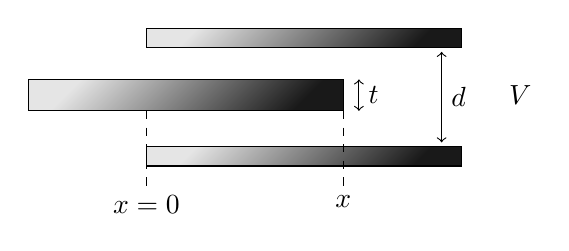
\begin{tikzpicture}
        \draw[black, shading=axis, right color=black!90, left color=black!10!white, shading angle=45, anchor=east, fill opacity=1] (1,1) -- (1,1.25) -- (-3,1.25) -- (-3,1) -- cycle;
        \draw[black, shading=axis, right color=black!90, left color=black!10!white, shading angle=45, anchor=east, fill opacity=1] (-0.5,0.6) -- (-0.5,0.2) -- (-4.5,0.2) -- (-4.5,0.6) -- cycle;
        \draw[black, shading=axis, right color=black!90, left color=black!10!white, shading angle=45, anchor=east, fill opacity=1] (1,-0.25) -- (1,-0.5) -- (-3,-0.5) -- (-3,-0.25) -- cycle;
        \draw[<->] (0.75,0.95) -- (0.75,-0.2) node[midway, right] {$d$};
        \draw[<->] (-0.3,0.6) -- (-0.3,0.2) node[midway, right] {$t$};
        \draw[dashed] (-0.5,0.2) -- (-0.5,-0.75) node[anchor=north] {$x$};
        \draw[dashed] (-3,0.2) -- (-3,-0.75) node[anchor=north] {$x = 0$};
        \node at (1.75,0.4) (v) {$V$};
\end{tikzpicture}\]


    First, we tackle the left side, where the sheet is being inserted in. Here, the capacitor has equivalent capacitance:

    \[ \frac{1}{C_{eq}} = \frac{1}{C_1} + \frac{1}{C_2} \]

    And for each of the capacitors we have $C = \frac{\varepsilon_0 A}{d}$ so:

    \begin{align*}
        \frac{1}{C_{eq1}} &= \frac{1}{\frac{\varepsilon_0 x L}{\frac{d-t}{2}}} + \frac{1}{\frac{\varepsilon_0 x L}{\frac{d-t}{2}}}\\
        &= \frac{d-t}{2\varepsilon_0 xL} + \frac{d-t}{2\varepsilon_0 xL}\\
        &= \frac{d-t}{\varepsilon_0 xL}\\
        \therefore C_{eq1} &= \frac{\varepsilon_0 xL}{d-t}
    \end{align*}

    Since the other side has no metal sheet inserted into it, we then have:

    \[ C_2 = \frac{\varepsilon_0 (w-x)L}{d}\]

    Now since they are connected in parallel we have the total capacitance: 

    \[ C_{eq} = \frac{\varepsilon_0 xL}{d-t} + \frac{\varepsilon_0 (w-x) L}{d}\]

    This means that the potential difference then is equal to:

    \begin{align*}
        \Delta U &= \frac{1}{2} V^2 \varepsilon_0 L\left(\frac{x}{d-t} + \frac{w-x}{d}\right) \\
        &= \frac{1}{2} L V^2 \varepsilon_0\left(\frac{x}{d} - \frac{x}{d-t}\right)
    \end{align*}

    Notice that this $\Delta U$ is negative, implying that the final potential of the capacitor is higher than the initial. Under a closed system, this violates the law of conservation of energy, but because this system isn't closed (energy is constantly being supplied by the battery), this negative result actually makes complete sense. So to find the total work done by the external force, we use the formula $F = -\dfrac{dU}{dx}$:
    
    
    \begin{align*}
        F  &= -\frac{dU}{dx}\\
        &= -\frac{1}{2}\varepsilon_0 LV^2\left(\frac{1}{d} - \frac{1}{d-t}\right)\\
        &= -\frac{1}{2}\varepsilon_0 LV^2\left(\frac{t}{d(d-t)}\right) 
    \end{align*}

    % TODO: Check this solution - does it make sense that force is independent of position?
    

    \section{Problem 5}

    \subsection{Part a}
    
    There is no charge outside of the conductor (by construction), and thus we conclude that $\rho(r) = 0$ outside the conductor. From Poisson's equation:

    \[ \nabla^2 \delta V(r) = \frac{\delta \rho(r)}{\varepsilon_0}\]

    Since $\rho(r) = 0$ outside the conductor, then $\delta V(r)$ is also zero outside the conductor. Inside the conductor, we are assuming a constant potential (by the problem statment), and thus $\delta V(r) = 0$. As a result of this, we also have $\rho(r) = \text{constant}$, and thus $\delta \rho(r) = 0$. 

    Now due to the nature of perfect conductors, we know that there cannot be any $\vec{E}$ field within the conductor (otherwise, it would no longer be considered a perfect conductor). Thus, the charge must lie on the boundary of the surface. 

    Since the charge lies on the boundary, then the integral over all space will be zero since the charges on the surface do not contribute towards the volume integral.\footnote{Aren mentioned the fact that we're integrating over a surface with measure 0, so the Lebesgue integral over that space is also zero.}

    \subsection{Part b}

    To show that this formula is true, all we need to do is to show that all three of these terms are ways to express potential energy. We will use the following relationship:

    \[ \vec{E}(r) = -\nabla V(r) = \nabla V^*(r + \delta r)\]

    Using this relationship, we've proven that:

    \[ \frac{\varepsilon_0}{2} \int |\vec{E}|^2 d^3 r= \frac{\varepsilon_0}{2} \int |-\nabla V(r)|^2 d^3r = \frac{\varepsilon_0}{2}\int|\nabla(V^* + \delta V)|^2 d^3 r\]
    
    And since our basic relationsihp of $\dfrac{\varepsilon_0}{2}\int |\vec{E}|^2 d^3 r$ is an expression for energy, then the other two terms derived from it are also terms for energy. Thus, since all three terms in the sequence are representations of energy it makes sense that the sum of all three would equal the total potential energy of the system. $\blacksquare$ 

    \subsection{Part c}

    Consider the product rule mentioned in lecture:
    \[ \nabla (\phi \nabla \psi) = \phi \nabla^2 \psi  + \nabla \phi \nabla \psi\]

    And we isolate for the second term on the right hand side ($\nabla \phi \nabla \psi$) to get:
    
    \[ \nabla \phi \nabla \psi = \nabla(\phi \nabla \psi) - \phi \nabla^2 \psi\]

    Now we integrate on both sides to get the formula for the integration by parts for vector functions:

    \[ \int \nabla \phi \nabla \psi = \int \nabla (\phi \nabla \psi) - \phi \nabla^2 \psi\]

    Applying this to the second term in the problem statement:


    \[ \int \nabla V^*(r) \nabla \delta V(r) d^3r = \int \nabla(V^*(r) \nabla \delta V(r)) - V^*(r)\nabla^2 \delta V(r) d^3r\]

    Notice here that $\nabla \delta V(r) = 0$ because $\delta V(r) = 0$. (from part a), and thus both terms on the right hand side vanish to zero, making the entire integral equal to zero.

    \subsection{Part d}

    If we perturb the system, then $\delta V$ now becomes nonzero, making $|\delta V(r)|^2 > 0$. This means that any perturbation of the system will increase the energy of the system, proving what was asked in the problem statement. 

    When we solved the problem, we assumed that perturbation is defined such that a simple rearrangement of charges that causes the final result to be indistinguishable from the inital is not a perturbation.


    \section{Problem 6}

    \subsection{Part a}

    Like all the problems we've been doing with electric field, we separate this into two cases, $x < l$ and $x > l$. First we take the case where $x > l$, and use Gauss' law:

    \begin{align*}
        \oint \vec{E} \cdot d\vec{A} &= \frac{Q_{enc}}{\varepsilon_0}\\
        E(x) 2\pi r^2 &= \frac{\pi r^2 (2l)\rho}{\varepsilon_0}\\
        \therefore E(x) &= \frac{l\rho}{\varepsilon_0} 
    \end{align*}

    Same thing with $x < l$:

    \begin{align*}
        E(x) \cdot 2\pi r^2 &= \frac{\pi r^2 (2x)\rho}{\varepsilon_0}\\
        \therefore E(x) &= \frac{x\rho}{\varepsilon_0}
    \end{align*}

    \subsection{Part b}

    From the problem statement we're asked to take $\Phi(0) = 0$. We take the integral separately since we have different values of $E(r)$ for locations inside and outside the cylinder. Let's take $x < R$ first:

    \begin{align*}
        \Phi(x) - \Phi(0) &= -\int_0^x E(x) dx\\
        \Phi(x) &= -\int_0^x \frac{x\rho}{\varepsilon_0} dx\\
        &= -\frac{\rho x^2}{2\varepsilon_0}
    \end{align*}

    Now to calculate the potential for $x > R$, we need to evaluate $\Phi(l)$:

    \[ \Phi(l) = -\frac{\rho l^2}{2\varepsilon_0}\]

    Now we take the integral for points $x > l$: 

    \begin{align*}
        \Phi(x) - \Phi(l) &= -\int_l^x \frac{\rho l}{\varepsilon_0} dx + \Phi(l)\\
        &= \left[\frac{l\rho x}{\varepsilon_0}\right]_x^l - \frac{\rho l^2}{2\varepsilon_0}\\
        &= \frac{l\rho (l-x)}{\varepsilon_0} - \frac{\rho l^2}{2\varepsilon_0}\\
        &= \frac{\rho l (l - 2x)}{2\varepsilon_0}
    \end{align*}

    %Comment about this


    \subsection{Part c}

    This part of the problem just asks us to verify Poisson's and the differential form of Gauss' law. Verifying Gauss' law first:

    \[\rho(x) = \varepsilon_0 \nabla \cdot \vec{E}(\vec{r})\]

    The important thing to notice here is that our formula for $\vec{E}(\vec{r})$ is only one-dimensional, meaning that the partial derivatives can essentially be simplified to a single derivative:

    \begin{align*}
        \frac{\partial E}{\partial x} = \frac{dE}{dx} &= \frac{d}{dx}\left(\frac{x\rho}{\varepsilon_0}\right)\\
        &=\frac{\rho}{\varepsilon_0}
    \end{align*}
    Which confirms Gauss' law. Now for Poisson's equation: 

    \[ -\nabla^2 \Phi(r) = \frac{\rho}{\varepsilon_0}\]

    Note that for points outside of the cylinder, we then have $\nabla \cdot \vec{E}(r) = 0$, implying that $\rho(r) = 0$. This is consistent with our theory since we already know that $\rho(r) = 0$ outside of the cylinder.

    \medskip

    Similar to Gauss' law, since potential is also one dimensional our partial derivative is the same as evaluating a single derivative. First we verify this formula for $x < l$:

    \[\frac{\partial^2 \Phi(x)}{\partial x^2} = \frac{-\rho}{\varepsilon_0}\]

    Again, we have $\nabla^2 \Phi(x) = 0$ outside the cylinder, again makes perfect sense since $\rho(r) = 0$ outside of the cylinder.


    \section{Problem 7}

    The problem asks us to take the vector function defined in problem 2.31:
    \[ \begin{cases}
        E_x = 6xy\\
        E_y = 3x^2 -3y^2\\
        E_z z= 0
    \end{cases}\]

    All we need to do is calculate $\vec{\nabla}\times \vec{E}$:

    \begin{align*}
        \vec{\nabla}\times \vec{E} &= \begin{vmatrix}
            \hat \imath & \hat \jmath & \hat k \\
            \frac{\partial}{\partial x} & \frac{\partial}{\partial y} & \frac{\partial}{\partial z} \\
            E_x & E_y & E_z 
            \end{vmatrix}\\
            &= \hat \imath\left(\frac{\partial}{\partial y} E_z - \frac{\partial }{\partial z} E_y\right) - \hat \jmath \left(\frac{\partial}{\partial x} E_z - \frac{\partial}{\partial z} E_x\right) + \hat k \left(\frac{\partial}{\partial x}E_y - \frac{\partial}{\partial y} E_x \right)\\
            &= \hat\imath (0) - \hat\jmath (0) + \hat k (6x - 6x) = \vec{0} 
    \end{align*}

    Since the curl of the vector field is zero, then the entire vector field can be an electrostatic field. Evaluating the divergence of the field:

    \begin{align*}
        \nabla \cdot \vec{E} &= \frac{\partial E}{\partial x} + \frac{\partial E}{\partial y} + \frac{\partial E}{\partial z}\\
        &= \frac{\partial}{\partial x} (6xy) + \frac{\partial}{\partial y} (3x^2 - 3y^2) + \frac{\partial}{\partial z} 0\\
        &= 0
    \end{align*}

    \section{Problem 8} 

    \subsection{Grounding the outside shell}

    Since the system is already in static equilibrium (with the inner and outer shell having charge $+Q$ and $-Q$ respectively), there is no effect from adding a ground since the charges don't need to move anyways. 

    Another way to express this is the fact that if there were charge leaving the outer shell, then there would be an $\vec{E}$ field created outside the shell, and this will induce charge to enter the outer shell. The same argument can be applied if we have too much charge on the outer shell $-$ there would still be an $\vec{E}$ field induced on the outside of the shell, causing the charge to leave the shell.

    \subsection{Grounding the inside shell}

    Let the final charge on the inner shell be $Q_{f}$. Then via Gauss' law, we can show that: 

    \[ E(r) = \frac{Q_f}{4\pi r^2\varepsilon_0}\]

    Thus the potential is:
     
    \begin{align*}
        \Phi (R_1) - \Phi(R_2) &= -\int_{R_2}^{R_1} E(r) dr\\
        &= -\int_{R_2}^{R_1} \frac{Q_f}{4\pi r^2 \varepsilon_0} dr\\
        &= \frac{Q_f}{4\pi \varepsilon_0} \cdot \left[\frac{1}{r}\right]_{R_1}^{R_2}\\
        &= \frac{Q_f}{4\pi \varepsilon_0}\left(\frac{1}{R_2} - \frac{1}{R_1}\right)
    \end{align*}

    The potential at the outer shell must equal the potential outside the shell. This is due to Poisson's equation, where the potential at infinity must equal the potential at any point outside of the shell.\footnote{You could argue this with Gauss' law as well, saying that the $\vec{E}$ field must be constant since the enclosed charge is always the same.} So using this property, we have:

    \[ \frac{Q_f}{4\pi \varepsilon_0}\left(\frac{1}{R_2} - \frac{1}{R_1}\right) = \frac{-Q + Q_f}{4\pi \varepsilon_0 R_2}\]

    This leads to the solution:

    \[ Q_f = \frac{R_1}{R_2} Q\]

    \section{Problem 9}

    \subsection{Part a}

    To solve this problem, we solve for the potential difference from $R_1$ to $R_2$, then from $R_2$ to $R_3$. I'm going to spare the calculations since we've done this already in Problem 8, but here are the formulas for potential: 


    \[ \begin{cases}
        \Phi (R_2) - \Phi(R_1) = \frac{Q_1}{4\pi \varepsilon_0} \left(\frac{1}{R} - \frac{1}{2R}\right)\\
        \Phi(R_3) - \Phi(R_2) = \frac{Q - Q_1}{4\pi\varepsilon_0}\left(\frac{1}{2R} - \frac{1}{3R}\right)
    \end{cases}\]

    Since the inner and outer plates have to be of equal potential, then we can equate the two: 

    \[\frac{Q_1}{4\pi \varepsilon_0} \left(\frac{1}{R} - \frac{1}{2R}\right) = \frac{Q - Q_1}{4\pi\varepsilon_0}\left(\frac{1}{2R} - \frac{1}{3R}\right)\]

    Now solving for $Q_1$:

    \[ Q_1 = \frac{1}{4} Q \implies Q_3 = \frac{3}{4} Q\]

    We can draw this implication since the $\vec{E}$ field outside of the shells must be zero, and the only way to do that is with a net zero charge. Thus, the two charges must sum to $Q$.
    

    \subsection{Part b}

    We have three concentric shells at equipotential, so the total potential is: 

    \begin{align*} 
        V = 2\frac{Q_1}{2\pi \varepsilon_0} \left(\frac{1}{R} - \frac{1}{2R}\right) &= \frac{Q_1}{4\pi \varepsilon_0}\left(\frac{1}{R} - \frac{1}{2R}\right)\\
        &= \frac{Q_1}{4\pi \varepsilon_0} \left(\frac{1}{2R}\right)\\
        &= \frac{Q}{16\pi \varepsilon_0 R}
    \end{align*}

    Now using $C = \dfrac{Q}{V}$:

    \begin{align*}
        C &= \frac{Q}{\frac{Q}{16\pi \varepsilon_0 R}}\\
        &= 16\pi \varepsilon_0 R
    \end{align*}

    \subsection{Part c}

    Nothing will happen to the shells here because the battery is disconnected, and there's no way for this additional charge $q$ to move. So the only thing that happens is that the outer shell gains a charge $q$.
    
    \section{Problem 10}

    For a capacitor made of two cylinders, we have, from problem 2:
    \[\begin{cases*}
        V = \frac{\sigma a}{\varepsilon_0} \ln \left|\frac{b}{a}\right|\\
        C = \frac{Q\varepsilon_0}{\sigma a\ln\left|\frac{b}{a}\right|}
    \end{cases*}\]

    I've modified the formula for capacitance slightly since we don't have values of $L$ as in problem 2, by replacing it with a $Q$ and reverting the cancellations we had in that problem. Note that the $\sigma$ really doesn't matter too much here since it's just a constant for any given capacitor.

    Using $U = \frac{1}{2} CV^2$

    \begin{align*}
        U &= \frac{1}{2}\left(\frac{Q\varepsilon_0}{\sigma a\ln \left|\frac{b}{a}\right|}\right)\left(\frac{\sigma a}{\varepsilon_0} \ln \left|\frac{b}{a}\right|\right)^2\\
        &= \frac{1}{2}\frac{Q\sigma a}{\varepsilon_0}\ln \left|\frac{b}{a}\right|
    \end{align*}

    A lot of these terms are constants, so we can simplify this into the form:

    \[ U = A a \ln\left|\frac{b}{a}\right|\]

    where $A$ just represents the amalgamation of all those constants. To find the maximal distance, we can set $a = kb$ to get: 

    \[ U = A kb \ln \left|\frac{1}{k}\right|\]

    From here, we take a derivative and set it equal to zero to find the maximal value:

    \begin{align*}
        \frac{dU}{dk} = 0 &= -A(\ln(k)+1)\\
        \ln k + 1 &= 0\\
        \ln k &= -1\\
        \therefore k &= \frac{1}{e}
    \end{align*}

    And thus we have that $a = \frac{b}{e}$ maximizes the potential.




\end{document}
